\section{One problem only: the Hodge round}\label{sec:hodgeround}

The runs of Section~\ref{sec:experiments} spread the network over five problems. This section points the whole of it at one, the Hodge conjecture in the form of \cite{BB26c}: the conjecture is equivalent to two statements about abelian varieties, (F2), that every Hodge class on an abelian variety outside the part $R(Y)$ reached from the known constructions is algebraic, and (F3$'$), that on every smooth projective variety the Hodge classes are those coming from abelian varieties, $\mathrm{Hdg}^{p}=\mathrm{Ab}^{p}$. The paper proves that the locus on which either statement holds is dense in every family and is either everything or meagre, and it builds for each statement the object that would decide it next and proves at which step the construction stops. Those stopping points are the five target points of Table~\ref{tab:hodgetargets}. The question for the network is whether, with every result of \cite{BB26c}, of the companion paper on Weil classes \cite{BMB26b} and of the literature in its library, and with the fourteen external sources of Section~\ref{ssec:hodgesources}, it produces one object that passes one target point. The measured quantity is the gap of Section~\ref{ssec:gapnumbers}: for each target point the number of open steps between the best checked composite and the point, together with the counts of composites checked, rejected and stopped. Everything in this section was fixed before the runs except the numbers.

\begin{table*}[t]
\caption{The five target points of the Hodge round, from \cite{BB26c}. Each is the object that paper needs next and could not build; ``open steps'' is the depth of the deepest open step in the library's route to the point, the gap of Fig.~\ref{fig:hodgerounds}(c). None is reached.}
\label{tab:hodgetargets}
\centering
\footnotesize
\setlength{\tabcolsep}{4pt}
\begin{tabular}{@{}p{0.12\textwidth}p{0.42\textwidth}p{0.30\textwidth}p{0.08\textwidth}@{}}
\toprule
\rr target & \rr object that passes it & \rr where \cite{BB26c} stops & \rr open steps \\
\midrule
\rr F2.lift & \rr for one polarised abelian scheme $A\to S$ with a flat Hodge class $\xi$ algebraic at a CM point $c$, a semiregular object at $c$ with Chern character $\xi_{c}$; then $\xi$ is algebraic on all of $S$ & \rr the CM point exists in every family; the semiregular object at it does not & \rr 3 \\
\rr F2.E06 & \rr a convolution $E$ of the pieces $O_{Z_{\zeta}}\otimes L^{k}[s]$, $L^{l}[t]$ on $E_{0}^{6}$, $E_{0}=\mathbf{C}/\mathbf{Z}[i]$, with $\mathrm{ch}(E)$ of polarised shape and $\dim\mathrm{Ext}^{2}(E,E)=57$ & \rr the $35$ pieces of its Proposition on separation give $\dim\mathrm{Ext}^{2}\ge2605$; four configurations are left open & \rr 2 \\
\rr F2.link & \rr one algebraic class $\xi\in\mathrm{Hom}_{\mathrm{Hdg}}(T_{X}(-1),T_{Z})$ on $X\times X\times Z_{K}$ for a Mumford fourfold $X$ whose cubic field $F$ contains no imaginary quadratic field & \rr $\mathrm{Hom}(X,Z_{K})=0$; the class is a Hodge class on a CM sixfold and nothing produces it & \rr 1 \\
\rr F3.cubic & \rr an algebraic correspondence of $S_{\lambda}$ (Picard number $13$, transcendental rank $9$) acting on $T(S_{\lambda})$ through the cubic field $F$, with $(F,D)$ not $(\mathbf{Q}(\zeta_{7})^{+},D_{\infty})$ or $(\mathbf{Q}(\zeta_{9})^{+},D_{\infty})$ & \rr finite groups reach only $\mathbf{Q}(\zeta_{7})^{+}$ and $\mathbf{Q}(\zeta_{9})^{+}$; a self-map $f$ with $f^{2}=n$ in $F$ forces $f\in\mathbf{Q}$ & \rr 1 \\
\rr F3.sqrt & \rr a family of K3 surfaces with real multiplication by $\mathbf{Q}(\sqrt{10})$ or $\mathbf{Q}(\sqrt{14})$ on which a chain of symplectic quotients or an isogeny of elliptic surfaces starts & \rr the chain theorem gives $\sqrt6$ and the Fricke cases; no family starts the chain for $\sqrt{10}$, $\sqrt{14}$ & \rr 1 \\
\bottomrule
\end{tabular}
\end{table*}

\subsection{Library, agents and rounds}\label{ssec:hodgerun}

The library for this round has $76$ typed constructions: the $19$ results of \cite{BB26c} that bear on the target points; $9$ of \cite{BMB26b}, namely Markman's theorem for trivial discriminant, the Weil tori, the convolutions on $E_{0}^{6}$ and on $E_{0}^{8}$, the quartic rank, the abelian covers, Schoen's product, the Vandermonde intersections and the escape theorem; $34$ results of the literature from Deligne to Markman's recent work, among them one unrefereed claim, the family of preprints in \cite{OAI26b} that asserts the Hodge conjecture for abelian varieties of CM type and for products of K3 surfaces, which enters as a hypothesis and never as a result; two counts computed for this round (Section~\ref{ssec:hodgecount}); six moves that change the variety (blow-up at a CM point, degeneration to a CM fibre, Kuga--Satake passage, fibration, Hilbert scheme, isogeny cover); and six open conjectures from the OpenConjecture collection (Section~\ref{ssec:hodgesources}), which the refuter treats as hypotheses, so that a composite resting on one is recorded as conditional and stopped. One agent sits on each target point. In a \emph{steady} round each agent runs six generations of ten pairings, with the refuter and the memory of Section~\ref{ssec:memory}; in a \emph{burst} each agent runs ten generations of forty pairings and the round then checks three hundred random chains of three to six constructions, pruned by the same refuter. Every checked composite is recorded with its verdict and its reason, so that no later round checks it again.

Rounds $1$ to $11$ were steady and round $12$ was a burst. Fig.~\ref{fig:hodgerounds} shows the run. The memory records $78$ checked composites in the first round, $29$ in the second, and between $7$ and $16$ in each of the next eight, as the combinations of the library are used up; round $11$, run after the two counts and the moves had entered the library, checked $35$. In all $230$ composites were checked in the eleven steady rounds, $22$ survived, and every survivor is a known result: the reduction to (F2) and (F3$'$), the propagation theorem, the density of CM points, Markman's theorem and the cases it covers. No composite reaches a target point, and the gap of every target point is the same after round $11$ as after round $1$: three open steps for F2.lift, two for F2.E06 and one for each of the other three.

Round $12$ had a time limit of $7000$ seconds. It committed $29$ checked composites to the memory in its first $98$ minutes and was stopped at the limit before it wrote its summary and before the long chains began. None of the $29$ survived. Twenty-four were stopped because they rest on an open conjecture used as a hypothesis, the derived form of the Hodge conjecture or a statement on generic Hodge classes from the OpenConjecture entries; three stopped at the count on $E_{0}^{6}$, one at the semiregular object of F2.lift, and one was rejected. Most of the time of the round went into the channel, which brought $58{,}872$ records of the memory to the proposers, against $11{,}558$ in round $11$ and between $1{,}546$ and $4{,}108$ in each earlier round. The burst therefore multiplies the cost of a round and moves the search toward composites that assume what they need; it does not change the gap. A wider search of the same library does not move a flat line at the depth of the first open step, because that step is not a combination of what the library holds.

\begin{figure*}[t]
\centering
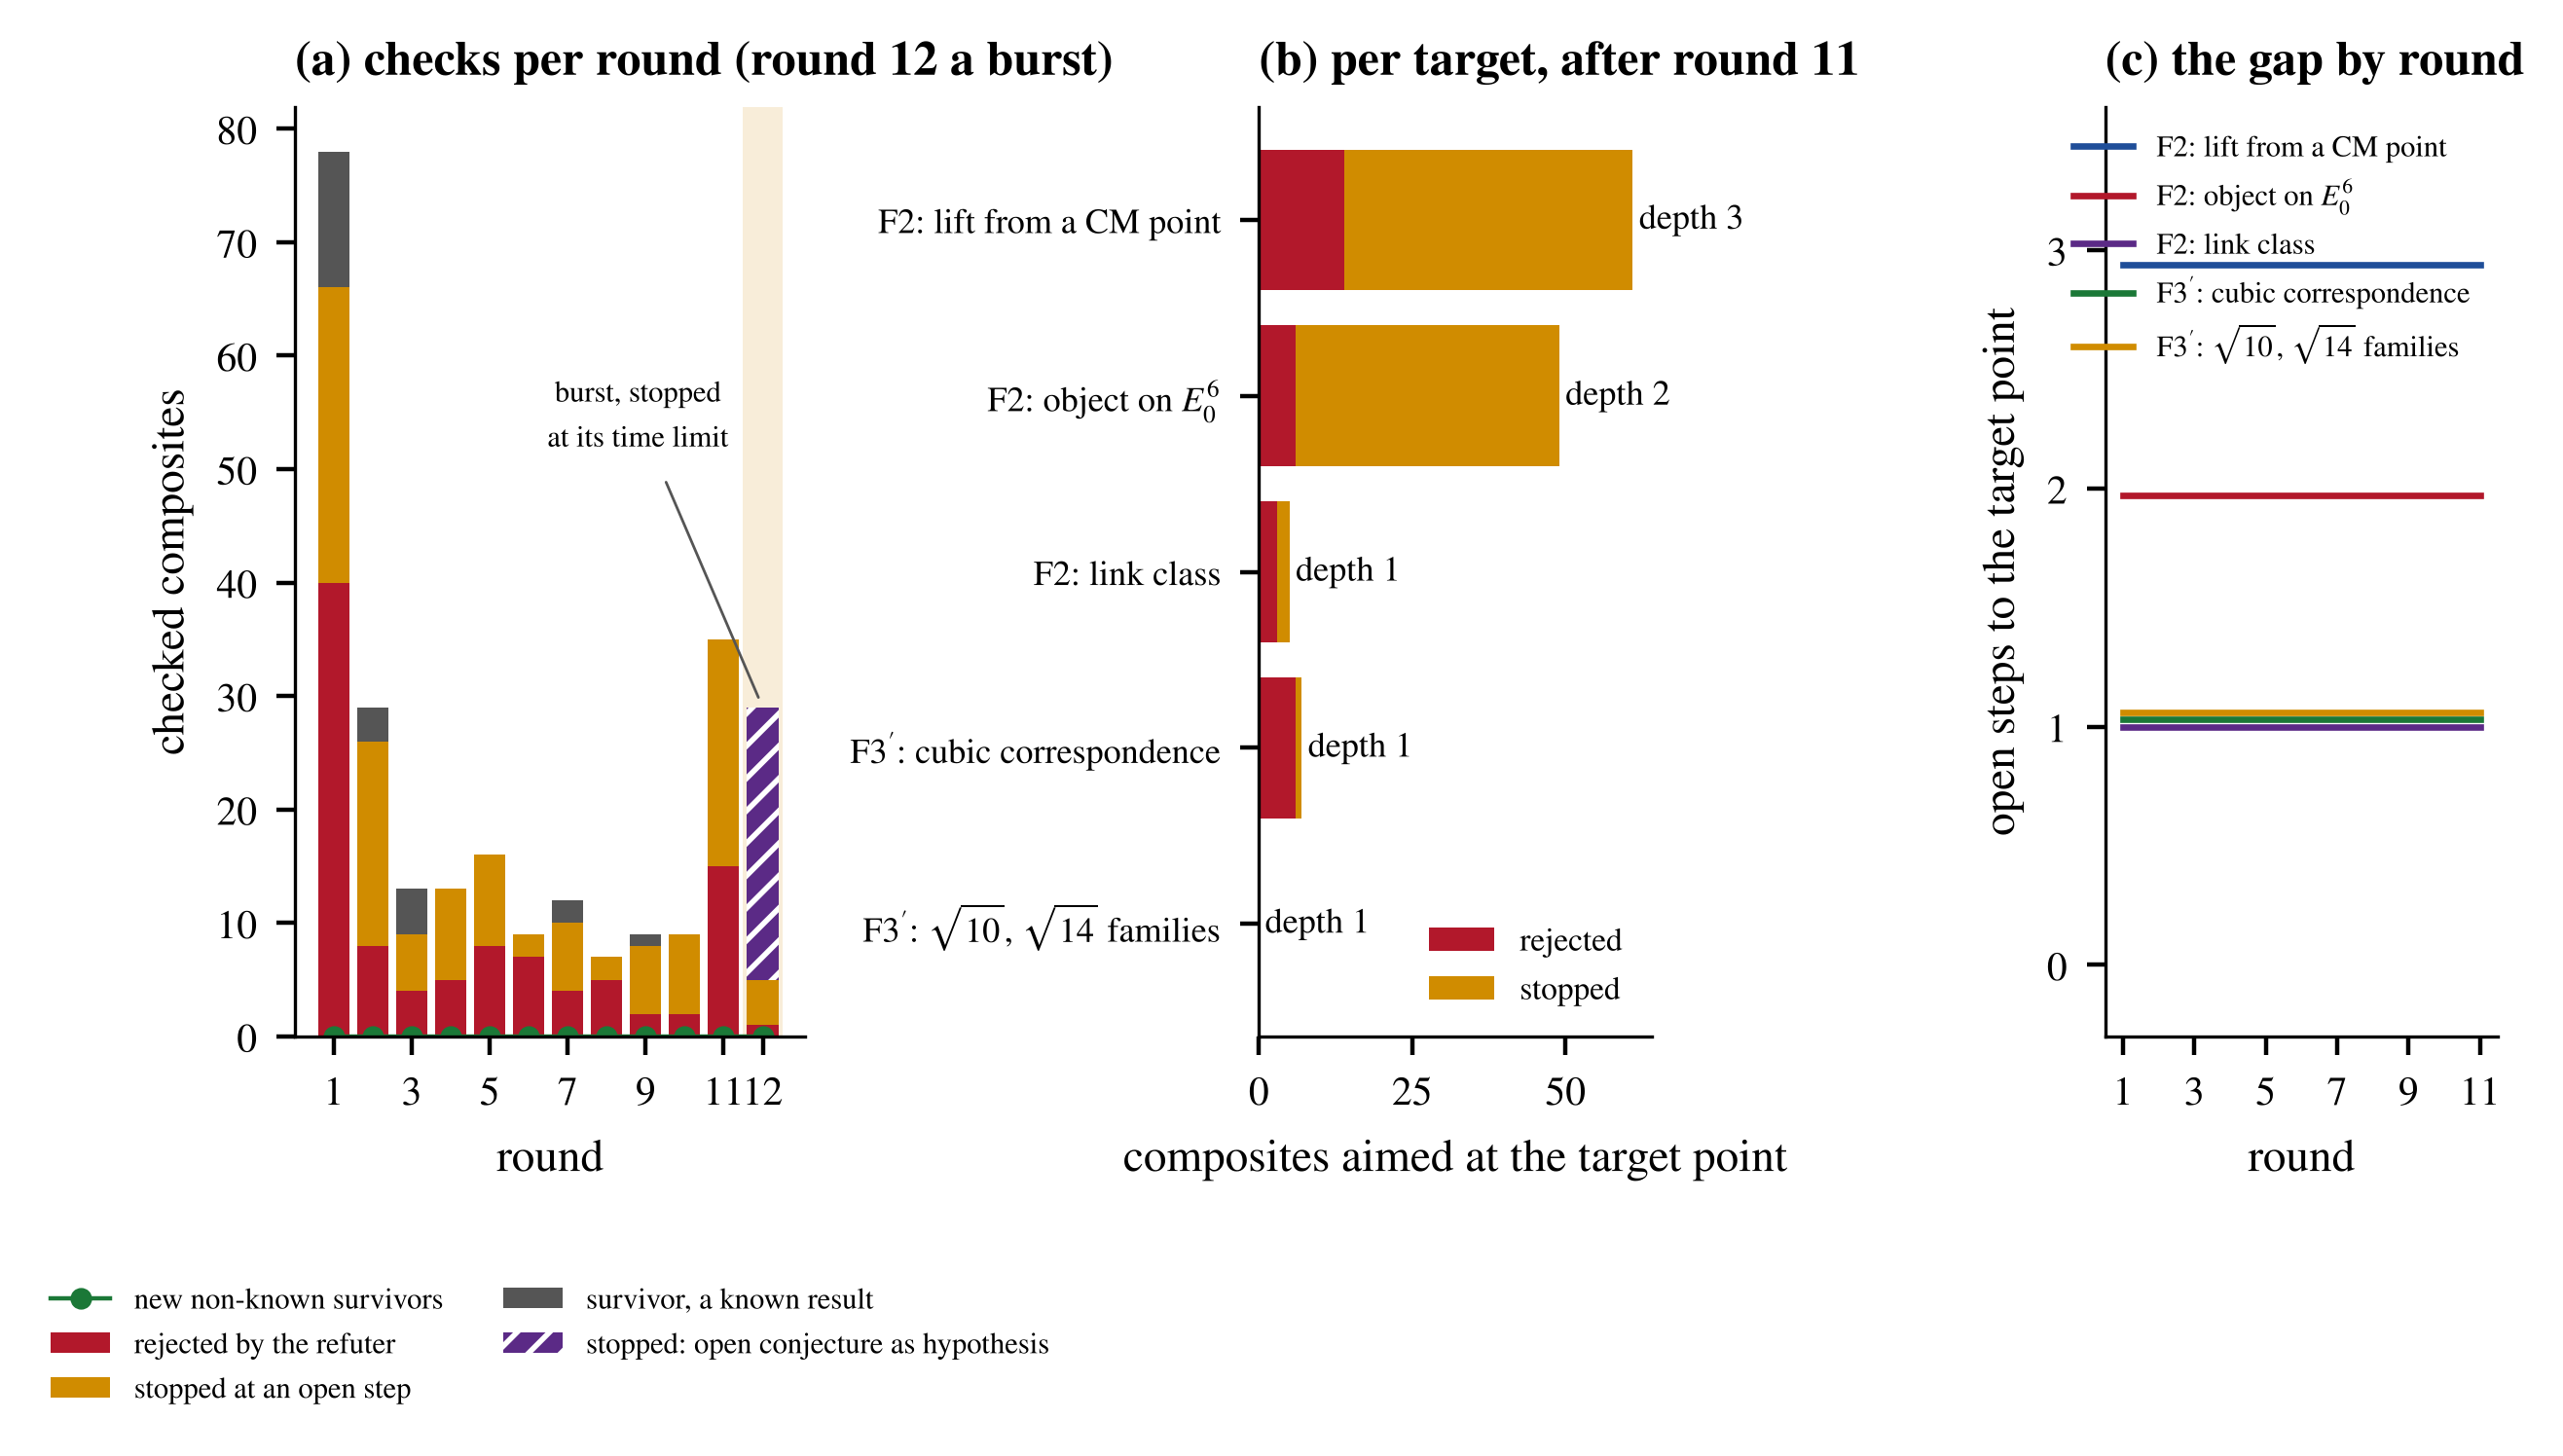
\includegraphics[width=0.98\textwidth]{figures/fig_hodgerounds}
\Description{Stacked bars of checked composites per round of the Hodge-only run: rejected, stopped at an open step, and survivors.}
\caption{The Hodge-only run. (a) Checked composites per round, from the memory: rejected by the refuter, stopped at an open step, and survivors, all of them known results; the green line, the survivors that are more than a known result, is zero in every round. Round $12$ (shaded) is the burst, stopped at its time limit; its hatched part rests on an open conjecture used as a hypothesis. (b) The composites aimed at each target point over rounds $1$ to $11$, with the depth of the gap after round $11$. (c) The gap of each target point by round: the number of open steps between the best checked composite and the point. It does not move.}
\label{fig:hodgerounds}
\end{figure*}

\subsection{Counting on \texorpdfstring{$E_{0}^{6}$}{E0\textasciicircum 6}}\label{ssec:hodgecount}

The target F2.E06 is the one that a finite computation can decide, and \cite{BB26c} leaves four configurations open after its $35$ pieces: (a) four or more line bundles, (b) one sheaf at two shifts, (c) one threefold at several twists, (d) two threefolds at the same shift meeting along an abelian surface. For a convolution $E$ of pieces $F_{a}$ the complex $\mathrm{Ext}^{\bullet}(E,E)$ is filtered by the blocks $\mathrm{Ext}^{k}(F_{a},F_{b})$ with total degree $k+s_{b}-s_{a}$, and $\dim\mathrm{Ext}^{2}(E,E)$ is at least the number of degree-two blocks that no differential reaches or leaves: a block $\mathrm{Ext}^{2}(F_{a},F_{b})$ is \emph{isolated} when no degree-one block maps to it along a chain of pieces and it maps to no degree-three block, and a bound that counts only isolated blocks is conservative, since a non-exact block can only add edges. The Ext groups of the pieces are the tables of \cite{BB26c} for $K=\mathbf{Q}(i)$, with $\chi_{Z_{\zeta}}=8$ and the groups between threefolds meeting along an abelian variety of dimension $d$ in $\prod_{j}\lvert\zeta_{j}-\zeta_{j}'\rvert^{2}$ components. We computed, for every polarised configuration of each family in a window of twists $1$ to $4$ and shifts $-3$ to $3$, the sums $C^{1},C^{2},C^{3}$ of the block dimensions by total degree, the Euler characteristic $C^{2}-C^{1}-C^{3}$, the isolated blocks, and a restricted Euler bound that removes the blocks that cannot interact. Fig.~\ref{fig:hodgepieces} shows the pieces of the least-bound configuration of family (a) and its block matrices; Fig.~\ref{fig:hodgebounds} shows the bounds over the families.

\begin{figure*}[p]
\centering
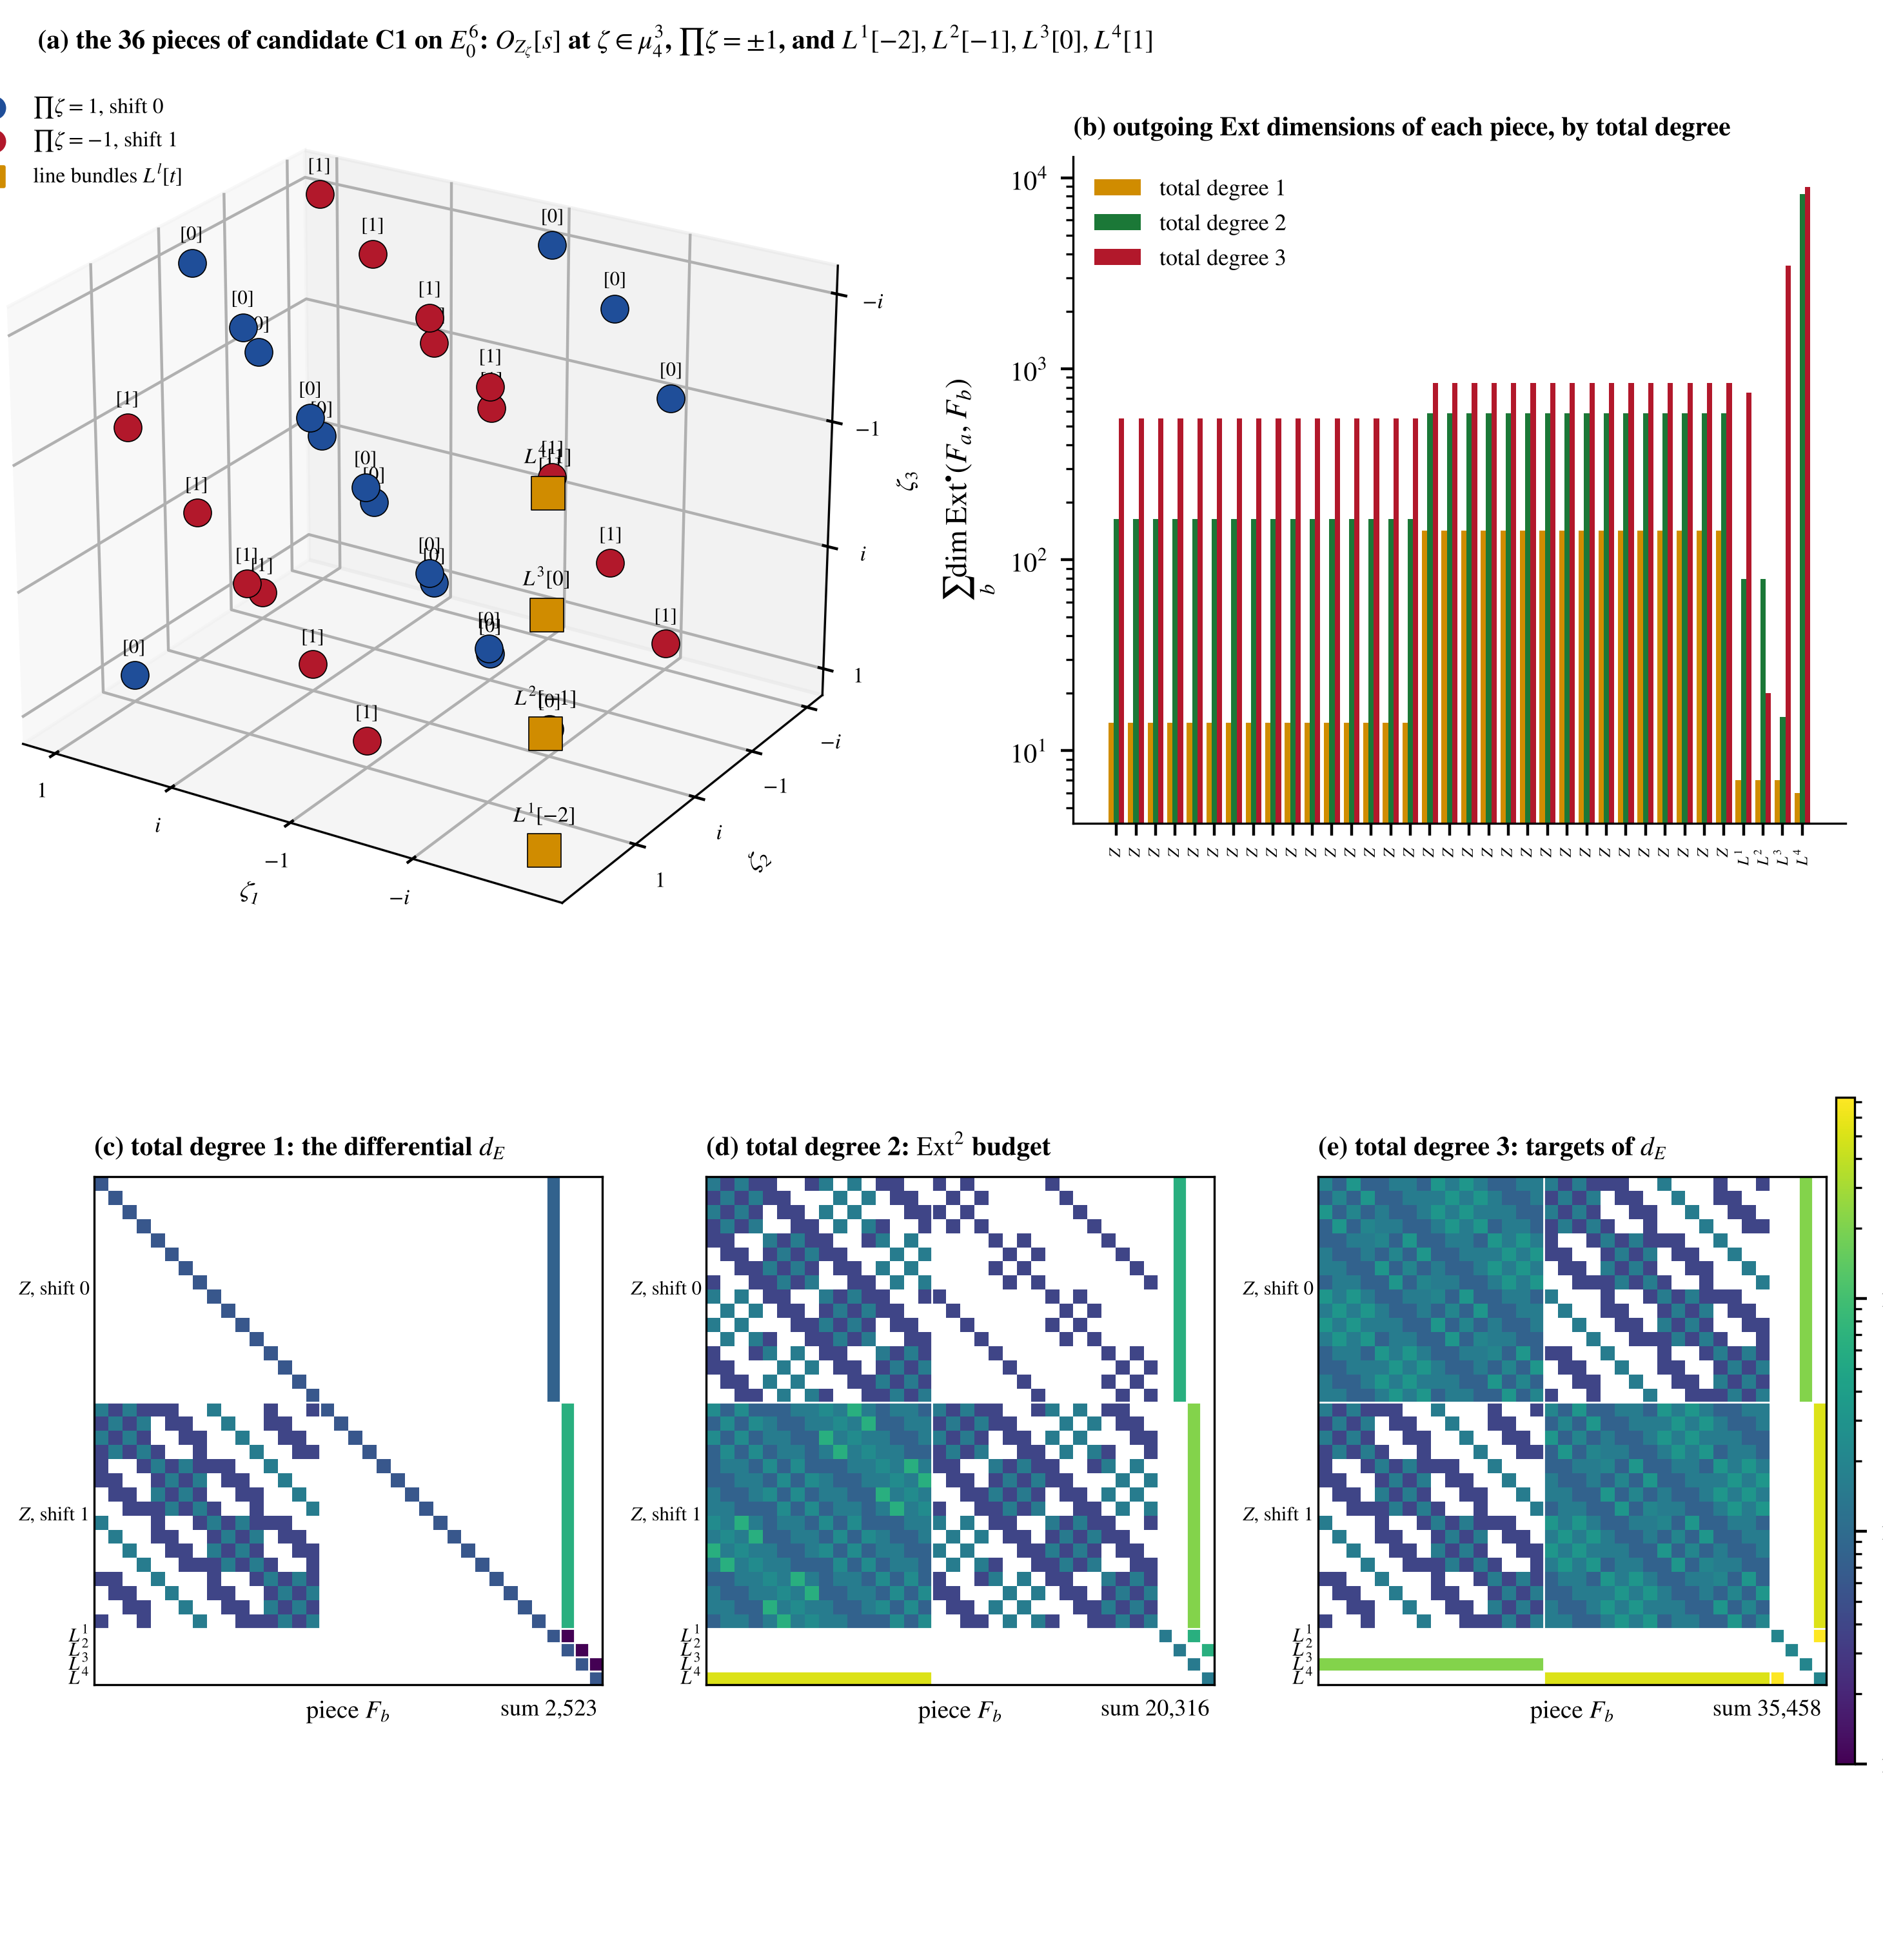
\includegraphics[width=0.98\textwidth,height=0.78\textheight,keepaspectratio]{figures/fig_hodgepieces}
\Description{Diagram of the thirty-two threefold pieces of candidate C1 on the sixfold and the blocks of their Ext groups.}
\caption{The pieces of candidate C1 on $E_{0}^{6}$ and their Ext blocks. (a) The $32$ threefold pieces $O_{Z_{\zeta}}[s]$ at the characters $\zeta\in\mu_{4}^{3}$ with $\prod\zeta=\pm1$, the sign fixing the shift, and the four line bundles $L^{1}[-2]$, $L^{2}[-1]$, $L^{3}[0]$, $L^{4}[1]$ of the least-bound configuration of family (a). (b) For each piece, the sum of the dimensions of the Ext groups to all pieces, by total degree. (c)--(e) The block matrices by total degree: the degree-one blocks carry the differential $d_{E}$, the degree-two blocks are the budget from which $\mathrm{Ext}^{2}(E,E)$ is cut, and the degree-three blocks are the targets of $d_{E}$ on degree two; the white lines separate the two parity classes of threefolds and the line bundles. Every degree-two block of this configuration is reached or leaves, so the counting bound is $0$ and the rank of the sixfold product decides.}
\label{fig:hodgepieces}
\end{figure*}

\begin{figure*}[t]
\centering
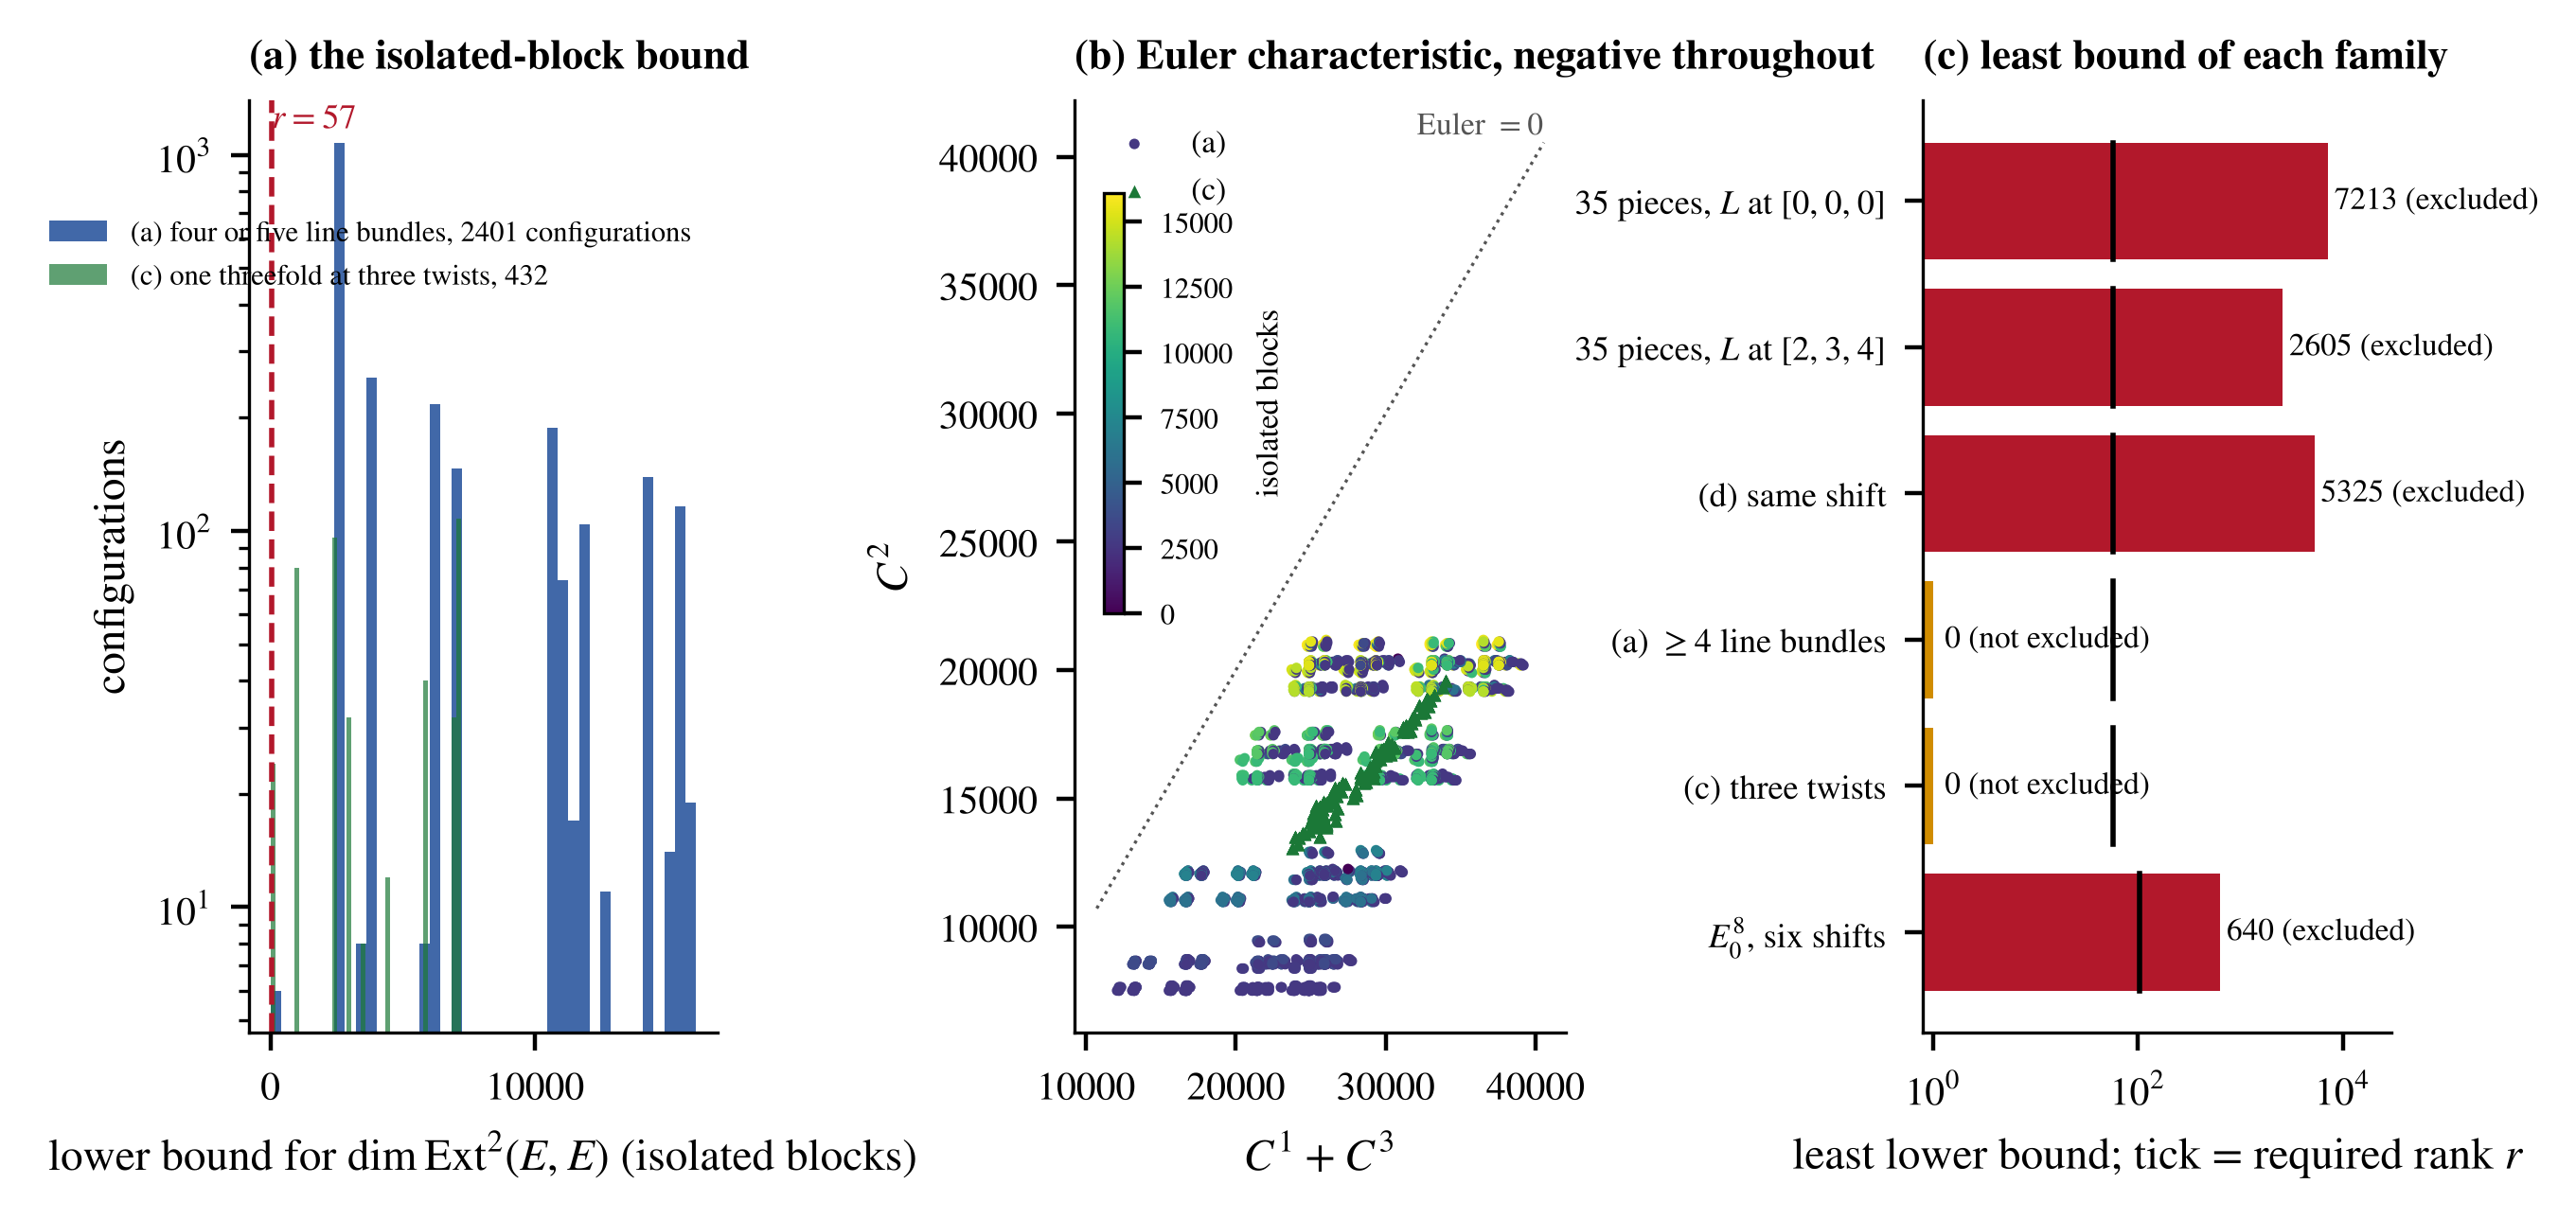
\includegraphics[width=0.98\textwidth]{figures/fig_hodgebounds}
\Description{Histograms of the isolated-block lower bound for the dimension of Ext squared over polarised configurations against the required rank 57, a scatter of Euler-characteristic terms, and the least bound of each family.}
\caption{Counting on $E_{0}^{6}$. (a) The isolated-block lower bound for $\dim\mathrm{Ext}^{2}(E,E)$ over the $2401$ polarised configurations of family (a) and the $432$ of family (c), against the required rank $r=57$. (b) $C^{2}$ against $C^{1}+C^{3}$ for the same configurations: the Euler characteristic is negative everywhere, so no configuration is excluded by it. (c) The least bound of each family against the rank it must meet: the $35$ pieces and family (d) are excluded, families (a) and (c) are not; the row for $E_{0}^{8}$ is the bound of \cite{BMB26b} within six shifts.}
\label{fig:hodgebounds}
\end{figure*}

The results are these. The $35$ pieces of \cite{BB26c} with the three line bundles at shifts $(0,0,0)$, $(2,3,4)$ or $(-3,-2,-1)$ have at least $7213$, $2605$ and $2605$ isolated degree-two blocks, so $\dim\mathrm{Ext}^{2}\ge2605>57$, in agreement with the bound $2560$ of \cite{BMB26b} for its line-bundle model. Family (d), two threefolds at the same shift meeting along a surface, has six polarised configurations in the window and the least bound is $5325$: it is excluded. Family (b) has no polarised configuration in the window. Family (a) has $2401$ polarised configurations, and for the four line bundles $L^{1}[-2],L^{2}[-1],L^{3}[0],L^{4}[1]$ the isolated blocks are $0$ and the Euler characteristic is $-17665$; family (c) has $432$, and for one threefold at the twists $1$ and $2$ at the shifts $-1,0,1,2$ the isolated blocks are again $0$. Counting decides nothing for (a) and (c), and what decides them is the shape of the closed chains of pieces along which a term of $d_{E}$ can return to a diagonal block. For (a) the shape alone suffices. The twisting cochain of a convolution is strictly upper triangular, so a diagonal component of $d_{E}(y)$ at a piece needs a closed chain through that piece with $y$ on one step and a nonzero component of the cochain on every other step; a threefold piece on no such chain keeps its diagonal class $\mathrm{ev}_{F}(v)$, which has rank $3$ on the nine directions of the Weil family, and the criterion fails. Counting Ext degrees around a chain shows that with at most five line bundles every closed chain through a threefold carries four or five of them, at consecutive shifts in the order of their exponents, and that its threefold pieces all sit at shifts of one parity. With five line bundles the Maurer--Cartan component between two of them two shifts apart is a product of two sections of powers of $L$, so of two consecutive steps one is zero, and at most one window of four carries chains. The Chern character pulls the other way: it has the polarised shape only if the threefold pieces at even and at odd shifts are equal in number and in total twist, because all the classes $[Z_{\zeta}]$ have the same component in the subring generated by the coordinate curves and that component is not a multiple of $\theta^{3}$. So some threefold lies on no chain, and every convolution of family (a) with at most five line bundles fails, for every choice of twists; the sixfold product on the chain of \cite{BB26c} is not needed. Two further facts carry the argument to seven line bundles. A chain contributes to the diagonal block only through its one step where the cochain vanishes, and if that step $b\to c$ follows a nonzero step $a\to b$ with $a\to b\to c$ the only path from $a$ to $c$, then the component of $d_{E}(y)$ from $a$ to $c$ is the product of the section on $a\to b$ with $y_{bc}$, while the Maurer--Cartan defect there vanishes; $A_{0}$ is integral, so $y_{bc}=0$ and the chain does nothing. And a chain climbs one shift at a time, so its line bundles fill an interval of shifts, and a configuration with an empty shift splits into pieces that do not interact. A search over every arrangement of at most eight line bundles whose shifts form an interval, $598427$ in all, finds that a piece with at most five line bundles carries no chain that acts, and one with six or seven carries such chains at one parity only. So every convolution of family (a) with at most seven line bundles fails. With eight, $31$ arrangements reach both parities, the typical one a tower with two line bundles at each of three middle shifts, where every Maurer--Cartan component has two paths; deciding them needs the ranks of the products along the chains, which the shape of the chains does not show. For (c) the chains have lengths two to five, and the ranks of $m_{3}$ to $m_{5}$ along them decide it.

\subsection{Candidates}\label{ssec:hodgecandidates}

Exclusion alone leaves a target point where it was, so the agents also construct. Table~\ref{tab:hodgecandidates} lists the eight explicit candidates, each with its invariants, what it achieves, where it falls short and what decides it; Fig.~\ref{fig:hodgemap} places them under their target points. Five die. C1, family (a) with four line bundles, has no closed chain through any of its threefolds and fails by the argument above. C3, the two threefolds at one shift, fails by the count above. The link class as a construction (C5) dies because a Hodge class on the CM sixfold $X\times X\times Z_{K}$ is exactly the statement to prove and $\mathrm{Hom}(X,Z_{K})=0$ leaves no map to transport it, so C5 survives only as the reduction it already is in \cite{BB26c}. The correspondences of $S_{\lambda}$ from Mukai vectors, Buskin's isometries and self-maps (C6) die because a self-map $f$ of the transcendental lattice with $f^{2}=n$ in a cubic field is rational, and the moduli-of-sheaves correspondences act through the Hodge isometries that \cite{BB26c} classifies. C7, a chain for $\sqrt{10}$ through a symplectic involution and a symplectic automorphism of order five, multiplier $2/5\equiv10$ modulo squares, dies by a rank count: the surfaces along a chain have the same transcendental space up to scaling, the coinvariant lattice of an automorphism of order five has rank $16$, so the transcendental lattice of $S'$ has rank at most five, while real multiplication by a real quadratic field needs rank at least six, a space of dimension two over the field having an abelian Hodge group and so complex multiplication. Three are open and each names what decides it: C8, the rest of family (a), fails up to seven line bundles and is decided at eight by the ranks of the products along the chains in $31$ arrangements of shifts; C2 by the ranks of $m_{3}$ to $m_{5}$ along its chains, in the theta-function model of \cite{BMB26b}; and the Weil family through $E_{0}^{6}$ (C4), which needs C8 or C2 first. None of the eight is a proof of anything, and the table says so for each.

\begin{table*}[t]
\caption{The explicit candidates of the Hodge round. The status names the computation or the result that settles the candidate; ``dies'' means excluded with the reason given, ``open'' means that a stated computation decides it and has not been done. No candidate reaches its target point.}
\label{tab:hodgecandidates}
\centering
\footnotesize
\setlength{\tabcolsep}{4pt}
\begin{tabular}{@{}p{0.03\textwidth}p{0.07\textwidth}p{0.36\textwidth}p{0.30\textwidth}p{0.16\textwidth}@{}}
\toprule
\rr & \rr target & \rr object & \rr invariants and where it falls short & \rr status \\
\midrule
\rr C1 & \rr F2.E06 & \rr the $32$ threefolds $O_{Z_{\zeta}}[s]$ and $L^{1}[-2],L^{2}[-1],L^{3}[0],L^{4}[1]$ on $E_{0}^{6}$ & \rr $\mathrm{ch}$ polarised with $N=32$, Hankel rank $3$, $r=57$; $C^{1},C^{2},C^{3}=2523,20316,35458$; isolated $0$; no closed chain through a threefold: a chain reaches one parity of shift, the Chern character needs both & \rr dies \\
\rr C8 & \rr F2.E06 & \rr the threefolds $O_{Z_{\zeta}}\otimes L^{k}[s]$, each once, with six or more line bundles & \rr as many threefold pieces at even as at odd shifts, with equal total twist; fails with at most seven line bundles & \rr open: products along the chains in $31$ arrangements of eight \\
\rr C2 & \rr F2.E06 & \rr one threefold $Z_{111}$ at the twists $1,1,2,2$ and shifts $-1,0,1,2$ with the $35$ pieces & \rr polarised, isolated $0$, Euler $-11423$; chains of lengths $2$ to $5$; the identity between the two copies contracts the pair, the zero map leaves the chains & \rr open: ranks of $m_{3}$ to $m_{5}$ \\
\rr C3 & \rr F2.E06 & \rr two threefolds meeting along an abelian surface at the same shift, with a cancelling pair & \rr six polarised configurations; isolated $\ge5325>57$ & \rr dies \\
\rr C4 & \rr F2.lift & \rr the Weil family of dimension $9$ through $A_{0}=E_{0}^{6}$ with the product object of \cite{BB26c} at the CM point & \rr the object at $A_{0}$ is a convolution of the pieces of C1; at trivial discriminant the result would be Markman's theorem again, and the non-trivial discriminant needs C8 or C2 first & \rr open: C8 and C2, then one discriminant \\
\rr C5 & \rr F2.link & \rr the class $\xi$ as a Hodge class on the CM sixfold $X\times X\times Z_{K}$ at a CM point & \rr it is the Hodge conjecture for that sixfold; $\mathrm{Hom}(X,Z_{K})=0$ gives no transport & \rr dies as a construction \\
\rr C6 & \rr F3.cubic & \rr correspondences of $S_{\lambda}$ from Mukai vectors, Buskin isometries and self-maps & \rr $f^{2}=n$ in a cubic field forces $f\in\mathbf{Q}$; the isometries are those classified in \cite{BB26c} & \rr dies \\
\rr C7 & \rr F3.sqrt & \rr $S\to Y\leftarrow S'$ through a symplectic involution and a symplectic automorphism of order $5$, multiplier $2/5\equiv10$ & \rr coinvariant rank of order five is $16$, transcendental rank $\le5$ under order five, while real multiplication needs rank $\ge6$ & \rr dies \\
\bottomrule
\end{tabular}
\end{table*}

\begin{figure*}[p]
\centering
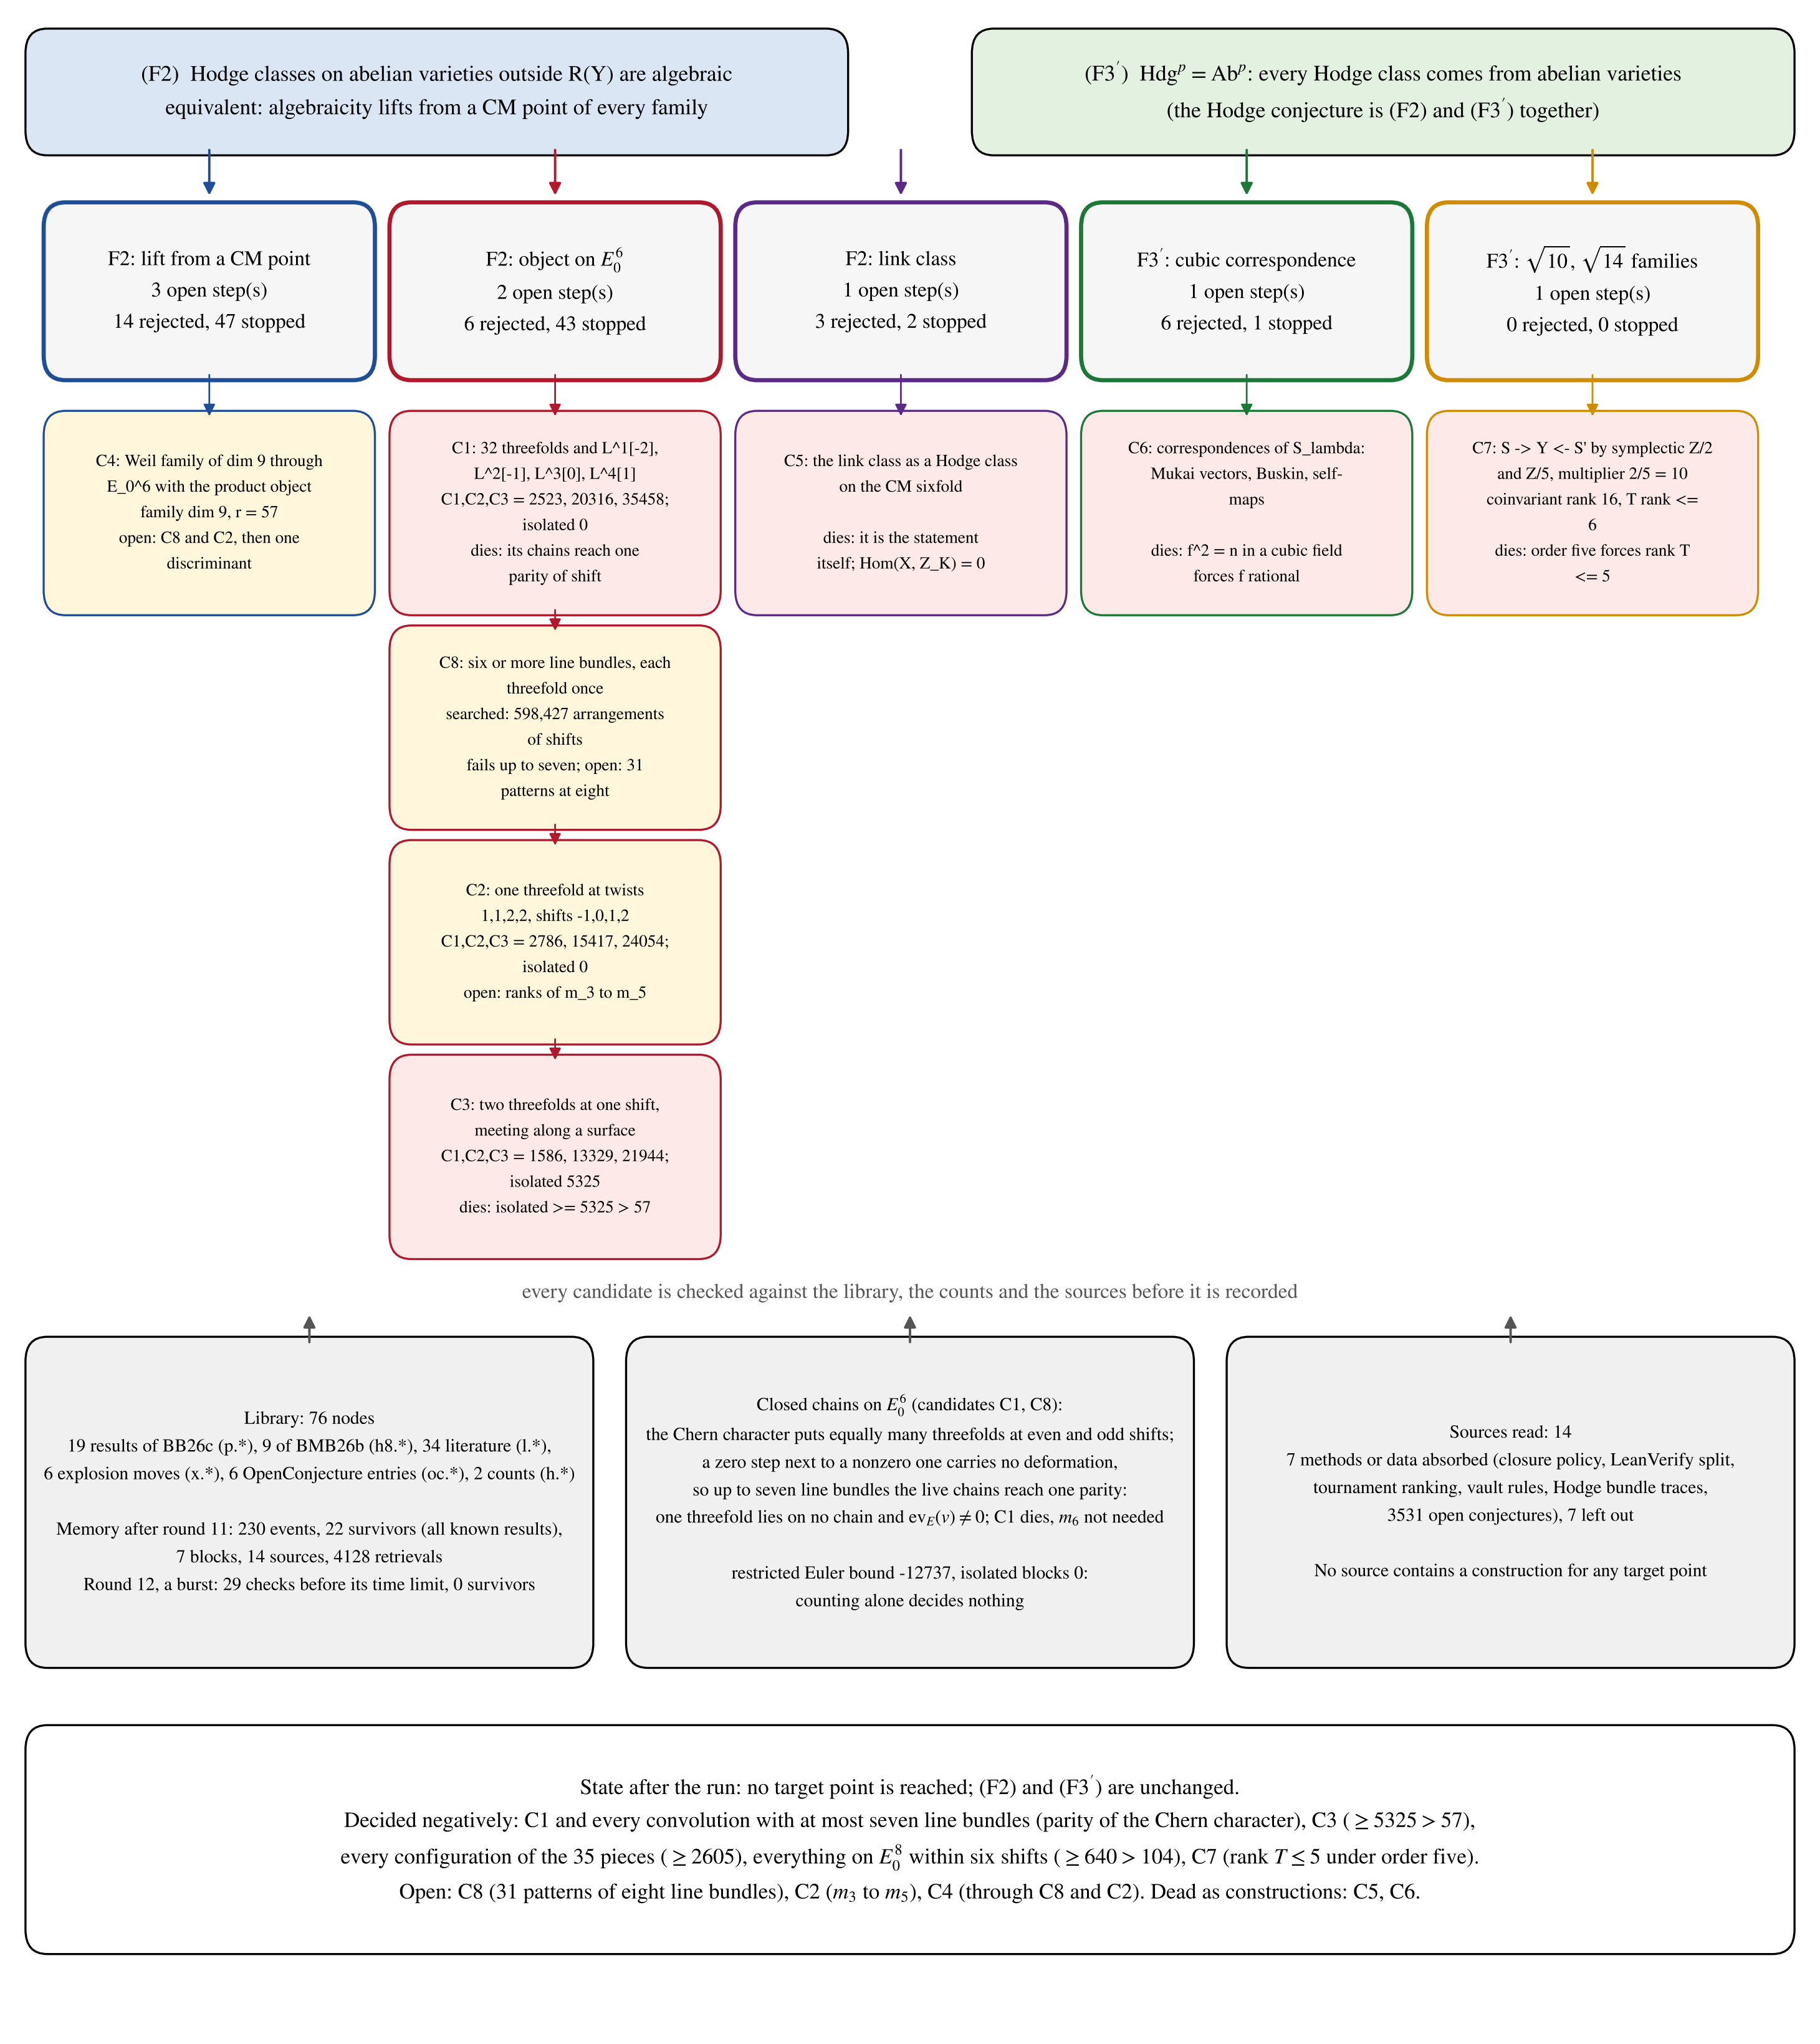
\includegraphics[width=0.98\textwidth,height=0.78\textheight,keepaspectratio]{figures/fig_hodgemap}
\Description{Map of the Hodge round: the two open statements at the top, the five target points with their gaps, and the eight candidates with their status.}
\caption{The map of the Hodge round. The two statements (F2) and (F3$'$) at the top, the five target points with their gap and their counts under them, the eight candidates under their targets (yellow open, red dead), and below them the three things every candidate is checked against before it is recorded: the library and the memory, the counting and chain results on $E_{0}^{6}$, and the fourteen sources. The bottom line is the state after the run.}
\label{fig:hodgemap}
\end{figure*}

\subsection{Sources}\label{ssec:hodgesources}

Fourteen sources were read during the round, and each is recorded in the memory with what was taken and what was left: a vault memory with embeddings and a knowledge graph, from which the community structure of the construction graph is kept and the server is not; a security reasoning stack with nothing for Hodge; an orchestration policy whose rule we adopt, that a problem is closed only after a kernel-checked Lean endpoint with an audited statement and the three standard axioms, never \texttt{native\_decide}, with evidence graded as lead, candidate, reproduced, formally verified and accepted; a Lean coding agent whose split of a theorem store from an axiom store the engine's Lean check follows; a hypothesis tournament whose Elo ranking orders the survivors of a burst; the output of a research agent on equivariant traces of the Hodge bundle over the moduli of curves, which enters as one construction; vault hygiene rules; four repositories with no mathematics; and the OpenConjecture collection of $3531$ open conjectures from the arXiv, in which a search finds $55$ on Hodge classes, abelian varieties, K3 surfaces and motives, six of which enter the library as conditional nodes. The memory shows that no source contains a construction for any target point; the ones that help change how the network keeps and ranks what it finds, not what it can find.

\subsection{What this round shows}\label{ssec:hodgeverdict}

Nothing closes. (F2) and (F3$'$) are where \cite{BB26c} left them, the gap of every target point is unchanged after the burst, and every decision is negative: the configuration (d) and every configuration of the $35$ pieces on $E_{0}^{6}$ are excluded by counting, every convolution of family (a) with at most seven line bundles by the parity of its chains against its Chern character, C7 by a rank count, two further candidates by arguments of \cite{BB26c} applied to them, and the sources add method and no construction. The decision on family (a) is the one the search did not reach: it comes from an argument by hand on the chains and the Chern character, not from a combination of library moves, and it replaces the sixfold Massey product of \cite{BB26c} by a parity count. What is left on $E_{0}^{6}$ is narrow and explicit: eight or more line bundles (C8), with $31$ arrangements of shifts at eight, and one threefold at several twists (C2), whose products $m_{3}$ to $m_{5}$ are a finite computation in the theta-function model of \cite{BMB26b}. The companion paper \cite{BMB26b} has carried out such computations for the fourfold products at distance two or more and for $E_{0}^{8}$ within six shifts, with the answer that they fail.
